%\documentclass{book}
\documentclass[12pt, a4paper, twoside, openright, titlepage]{book}
%-----------------------------------------------------------
%------------------------ packages -------------------------
%-----------------------------------------------------------
%\usepackage{caption2}
%\usepackage{tabu}  % added for long table
\usepackage{thesis}
\usepackage{comment}
\usepackage[hidelinks]{hyperref}
\usepackage{epsfig}
\usepackage[toc,page]{appendix}
\usepackage{algcompatible}
\usepackage{float}
\usepackage{color}
\usepackage{url}
\raggedbottom
\usepackage{fancyhdr}
\usepackage{array}
\usepackage{ctable}
\usepackage{multirow}
\usepackage{cite}
\usepackage{setspace}
\usepackage{longtable}
\usepackage{tocloft}
\usepackage{subfig}
\usepackage{epstopdf}
\usepackage{afterpage}
\usepackage{pdflscape}
\usepackage{epstopdf}

%\usepackage[cmex10]{amsmath}
\usepackage{amsmath}
%\usepackage{isomath}
\usepackage{cuted}
\usepackage{ae,aecompl}
%\usepackage[T1]{fontenc} % Was producing low-res fonts
%\usepackage{lmodern}
\usepackage{upgreek,bm}

\usepackage{amssymb}
\usepackage{array}
\usepackage{algorithm}
\usepackage{algpseudocode}

\usepackage{calligra}  %% used for fancy first letter

\newcolumntype{L}{>{\centering\arraybackslash}m{11cm}}
\newcolumntype{K}{>{\centering\arraybackslash}m{3cm}}
\newcolumntype{X}{>{\centering\arraybackslash}m{7cm}}
\newcolumntype{Y}{>{\centering\arraybackslash}m{4cm}}
\newcolumntype{W}{>{\centering\arraybackslash}m{6cm}}
\newcolumntype{M}[1]{>{\raggedleft\let\newline\\\arraybackslash\hspace{0pt}}m{#1}}
%-----------------------------------------------------------
%----------------------------- style -----------------------
%-----------------------------------------------------------
\pagestyle{fancy} \lhead{} \rhead{}
\fancyhead[LO]{\bfseries\rightmark}
\fancyhead[RE]{\bfseries\leftmark}
%\fancyfoot[RO,LE]{\thepage}
%\fancyhf{}			% Removes any previous fancyheader setting
%\oddsidemargin 0.5in \evensidemargin 0.2in
\oddsidemargin 0.5in \evensidemargin 0.0in
%\oddsidemargin 0.0in \evensidemargin 0.0in

\setcounter{secnumdepth}{3}
\setcounter{tocdepth}{3}



\newtheorem{thm}{Theorem}
\newtheorem{rem}{Remark}
\newtheorem{prf}{Proof}
\newtheorem{lem}{Lemma}

\DeclareMathOperator{\diag}{diag}

\newcommand{\thesisTitle}{Thesis Title}  % Input Thesis title
\newcommand{\authorName}{Author Name}  % Input Author name
\newcommand{\authorDept}{Department of <Department Name>}  % Input Department of Author
%-------------------------------------------------------------
%---------------------------- start --------------------------
%-------------------------------------------------------------
\begin{document}
%\pagenumbering{none}
    \setcounter{page}{1}
    \pagenumbering{roman}
    %----------------------------------------------------
%-------------------- cover page --------------------
%----------------------------------------------------
  %\pagestyle{empty} %%%%%%%%%%%%%%%%%%%%%%%%%%%%%%%%%%%%%%%%%%%%%%%%
\thispagestyle{plain}
\begin{center}
\vspace*{1cm} \begin{spacing} {1.25}

{\LARGE \bf \thesisTitle \\}

\end{spacing}
\end{center}



%\vspace{12cm}
\vspace{12cm}
\begin{flushright}
%\begin{Large}
\begin{Large}
{\bf {\em \authorName~~}\noindent \vskip -.8\baselineskip
\noindent \rule[-2.5 mm]{\textwidth}{3 pt}\\}
\end{Large}
%\end{huge}
\end{flushright}

  \cleardoublepage
  \setcounter{page}{1}
  \pagenumbering{roman}
%-----------------------------------------------------
%-------------------- Title --------------------------
%-----------------------------------------------------
   \phantomsection
   \addcontentsline{toc}{chapter}{Title Page}
   \thispagestyle{plain}
\begin{center}
\begin{spacing} {1.25}
{\LARGE \bf \thesisTitle}
\end{spacing}

\vspace*{2.0cm} {\em Thesis submitted to\\ Indian Institute of Technology, Kharagpur \\ 
for the award of the degree}\\
{\em of} \\
\vspace*{0.3cm}
{\Large {\bf Doctor\ \ of\ \ Philosophy}}\\
\vspace*{0.3cm}
{\em by}\\
\vspace*{0.3cm}
{\Large{\bf \authorName}}\\
\vspace*{0.3cm}
{\em under the supervision of }\\
\vspace*{0.2cm}
{\bf Prof. Supervisor 1}\\
\vspace*{0.1cm}
{\em and }\\
\vspace*{0.1cm}
{\bf Prof. Supervisor 2}\\
\vspace*{1cm}
\begin{figure}[htbp]
%  \centerline{\includegraphics{figure=iitlogo.pdf,height=4cm,width=3.5cm}}
  \centerline{\psfig{figure=IITLOGO.eps,height=4cm,width=3.5cm}}
\end{figure}
{{\bf \authorDept \\
INDIAN INSTITUTE OF TECHNOLOGY, KHARAGPUR\\
January 2021}} \\
\copyright 2021, \authorName. All rights reserved.
\end{center}
      
   \cleardoublepage
   \cfoot{\thepage}
   \begin{spacing}{1.1}
%-----------------------------------------------------
%-------------------- Approvalcert -------------------
%-----------------------------------------------------
   \phantomsection
   \addcontentsline{toc}{chapter}{Certificate of Approval}
    \thispagestyle{empty}
%\newgeometry{top=9cm, left=23mm, right=23mm}0.5in = 1.27
\newgeometry{top=5cm, left=26mm, right=20mm}
%\vspace{10cm}
%\begin{figure}[htbp]
%\includegraphics[width=2.5cm]{headTail/IITLOGOR}
%\end{figure}
%
%
%
%
%\vspace*{-4.0\baselineskip}
%
%\hspace*{2cm} {\large{\bf{\sf  Department of Electronics and Electrical Communication Engineering}}} \\
%\hspace*{2.6cm}   {\large{\bf{\sf Indian Institute of Technology, Kharagpur}}}\\
%\hspace*{2.6cm}   {\large{\sf Kharagpur, India 721302.}}\\
%\vspace*{0.5cm} \rule{\textwidth}{1.00pt}


%\hispagestyle{empty}

%\begin{figure}[htbp]
%  \psfig{figure=IITLOGO.eps,height=2.1cm,width=1.8cm}
%\end{figure}
%
%\vspace*{-4.0\baselineskip}
%
%\hspace*{2cm} {\large{\bf{\sf Department of Electrical Engineering}}} \\
%\hspace*{2.6cm}   {\large{\bf{\sf Indian Institute of Technology Kharagpur}}}\\
%\hspace*{2.6cm}   {\large{\sf Kharagpur, India 721302.}}\\
%\vspace*{0.5cm} \rule{\textwidth}{0.75pt}
\vskip 2.0\baselineskip \centerline{\underline{\Large{\bf APPROVAL
OF THE VIVA-VOCE BOARD}}} \vskip 2.0\baselineskip \noindent

\begin{flushright}
Date: January 5, 2020
%Date ___/___/_____
\end{flushright}
{\renewcommand{\baselinestretch}{2.0} Certified that the thesis entitled \textbf{\thesisTitle} submitted by \textbf{\authorName} to Indian Institute of Technology Kharagpur, for the award of the degree of Doctor of Philosophy has been accepted by the external examiners and that the student has successfully defended the thesis in the viva-voce examination held today.}\\
\vspace{1cm}
\begin{center}
\begin{table}[H]
\centering
\begin{tabular}{c c}
\_\_\_\_\_\_\_\_\_\_\_\_\_\_\_\_\_\_\_\_\_\_\_\_\_\_\_\_\_\_\_\_\_\_\_\_\_\_\_\_\_& \_\_\_\_\_\_\_\_\_\_\_\_\_\_\_\_\_\_\_\_\_\_\_\_\_\_\_\_\_\_\_\_\_\_\_\_\_\_\_\_\_\\
Prof. DSC 1 & Prof. DSC 2\\
(Member of the DSC) & (Member of the DSC)\\
\end{tabular}
\end{table}
\end{center}
\vspace{0cm}
\begin{center}
	\begin{table}[H]
		\centering
		\begin{tabular}{c}
			\_\_\_\_\_\_\_\_\_\_\_\_\_\_\_\_\_\_\_\_\_\_\_\_\_\_\_\_\_\_\_\_\_\_\_\_\_\_\_\_\_\\
			Prof. DSC 3\\
			(Member of the DSC)  \\
		\end{tabular}
	\end{table}
\end{center}

\vspace{0cm}
\begin{center}
\begin{table}[H]
\centering
\begin{tabular}{c c}
\_\_\_\_\_\_\_\_\_\_\_\_\_\_\_\_\_\_\_\_\_\_\_\_\_\_\_\_\_\_\_\_\_\_\_\_\_\_\_\_\_& \_\_\_\_\_\_\_\_\_\_\_\_\_\_\_\_\_\_\_\_\_\_\_\_\_\_\_\_\_\_\_\_\_\_\_\_\_\_\_\_\_\\
Prof. Supervisor 1 & Prof. Supervisor 2  \\
(Supervisor) & (Joint Supervisor)  \\
\end{tabular}
\end{table}
\end{center}
\vspace{0cm}
\begin{center}
\begin{table}[H]
\centering
\begin{tabular}{c c}
\_\_\_\_\_\_\_\_\_\_\_\_\_\_\_\_\_\_\_\_\_\_\_\_\_\_\_\_\_\_\_\_\_\_\_\_\_\_\_\_\_& \_\_\_\_\_\_\_\_\_\_\_\_\_\_\_\_\_\_\_\_\_\_\_\_\_\_\_\_\_\_\_\_\_\_\_\_\_\_\_\_\_\\
                    & (Prof. Chair DSC)  \\
(External Examiner) & (Chairman of the DSC)  \\
\end{tabular}
\end{table}
\end{center}

\restoregeometry


%\begin{flushleft}
%\raisebox{3mm}[2.5cm][0cm]{
%\begin{minipage}{4.8cm}
%Signature: \\
%Name: \\
%(Member of the DAC 1)\\
%\end{minipage}
%}
%\end{flushleft}
%
%\begin{center}
%\raisebox{1.2cm}[-2.5cm][0cm]{
%\begin{minipage}{4.8cm}
%Signature: \\
%Name: \\
%(Member of the DAC 2)\\
%\end{minipage}
%}
%\end{center}
%%
%
%%
%\begin{flushright}
%\raisebox{2.0cm}[-2.5cm][0cm]{
%\begin{minipage}{4.8cm}
%Signature: \\
%Name: \\
%(Member of the DAC 3)\\
%\end{minipage}
%}
%\end{flushright}
%
%\begin{flushleft}
%\raisebox{0cm}[2.5cm][0cm]{
%\begin{minipage}{4.8cm}
%Signature: \\
%Name: \\
%(Supervisor)\\
%\end{minipage}
%}
%\end{flushleft}
%
%\begin{flushright}
%\raisebox{1.0cm}[-2.5cm][0cm]{
%\begin{minipage}{4.8cm}
%Signature: \\
%Name: \\
%(Joint Supervisor)\\
%\end{minipage}
%}
%\end{flushright}
%
%
%\begin{flushleft}
%\raisebox{0cm}[2.5cm][0cm]{
%\begin{minipage}{4.8cm}
%Signature: \\
%Name: \\
%(External Examiner)\\
%\end{minipage}
%}
%\end{flushleft}
%
%
%\begin{flushright}
%\raisebox{9.0cm}[-2.5cm][0cm]{
%\begin{minipage}{4.8cm}
%Signature: \\
%Name: \\
%(Chairman)\\
%\end{minipage}
%}
%\end{flushright}
       
    \cleardoublepage
%------------------------------------------------------
%-------------------- Certificate ---------------------
%------------------------------------------------------
   \phantomsection
   \addcontentsline{toc}{chapter}{Certificate by the Supervisors}
   \thispagestyle{empty}

\begin{figure}[htbp]
  \psfig{figure=IITLOGO.eps,height=2.1cm,width=1.8cm}
\end{figure}

\vspace*{-4.0\baselineskip}

\hspace*{2cm} {\large{\bf{\sf \authorDept}}} \\
\hspace*{2.6cm}   {\large{\bf{\sf Indian Institute of Technology, Kharagpur}}}\\
\hspace*{2.6cm}   {\large{\sf Kharagpur, India 721302.}}\\
\vspace*{0.5cm}
\rule{\textwidth}{0.75pt}

\vskip 2.0\baselineskip \centerline{\underline{\Large{\bf
Certificate}}} \vskip 2.0\baselineskip \noindent This is to
certify that this thesis entitled {\bf \thesisTitle} submitted by {\bf \authorName}, to the Indian Institute of Technology Kharagpur, is a record of bonafide research work carried out under our supervision and is worthy of consideration for award of the degree of Doctor of Philosophy of the Institute.

\begin{flushright}
\raisebox{0.1cm}[3cm][0cm]{
\begin{minipage}{7.8cm}
{\bf Supervisor 1 }\\
Department of Supervisor \\
Indian Institute of Technology Kharagpur \\
{\sf India} 721302.
\end{minipage}
}
\end{flushright}
\vspace{1cm}
\begin{flushright}
\raisebox{0.4cm}[3cm][0cm]{
\begin{minipage}{7.8cm}
{\bf Supervisor 2}\\
  Department of Supervisor 2 \\
 Indian Institute of Technology Kharagpur \\
 {\sf India} 721302.\\
\end{minipage}
}
\end{flushright}

\ \\
Indian Institute of Technology Kharagpur, Kharagpur\\
Date:
%$~~~~~~$25$^{th}$ February, 2009       
   \cleardoublepage
%------------------------------------------------------
%-------------------- declaration ---------------------
%------------------------------------------------------
    \phantomsection
    \addcontentsline{toc}{chapter}{Declaration}
    \thispagestyle{empty}

%\vspace*{-4.0\baselineskip}

\vskip 2.0\baselineskip \centerline{\underline{\Large{\bf
Declaration}}} \vskip 2.0\baselineskip \noindent I certify that

\begin{itemize}

\item [a.] the work contained in the thesis is original and has
been done by me under the guidance of my supervisors;

\item [b.] the work has not been submitted to any other institute
for any other degree or diploma;

\item [c.] I have followed the guidelines provided by the Institute
in preparing the thesis;

\item [d.] I have conformed to ethical norms and guidelines while
writing the thesis;

\item [e.] whenever I have used materials (data, models, figures and text) from other
sources, I have given due credit to them by citing them in the text
of the thesis, and giving their details in the references, and taken
permission from the copyright owners of the sources, whenever
necessary.

\end{itemize}

\vspace{2cm} \authorName
     
    \cleardoublepage
%------------------------------------------------------
%--------------------- Dedication ---------------------
%------------------------------------------------------
    \thispagestyle{empty}%
\vspace*{0.25\textheight}
\begin{center}
{\AlgoFont{14} {Dedicated to}}\\
\vspace*{2.0\baselineskip}
{\AlgoFont{18} {\calligra My loving parents}}\\
\vspace*{0.5\baselineskip}
%{\AlgoFont{16} {\sf and}}\\
%\vspace*{0.5\baselineskip}
%{\AlgoFont{16} {\sf My grandmother who taught me happiness}}\\
\end{center}
    
    \cleardoublepage
%------------------------------------------------------
%--------------------- ack ----------------------------
%------------------------------------------------------
 
 \phantomsection
 \addcontentsline{toc}{chapter}{Acknowledgement}
 \chapter*{Acknowledgment}


%Finally, I would like to thank my family who always encouraged me for higher studies and made me believe that knowledge is more powerful than wealth. My deepest gratitude goes to my parents for their unflagging love and support throughout my life. 
            
 \cleardoublepage
%--------------------------------------------------------
%---------------------- Abstract ------------------------
%--------------------------------------------------------
\phantomsection
\addcontentsline{toc}{chapter}{Abstract}
%\newgeometry{top=2cm, left=40mm}
\chapter*{Abstract} %\vspace{-5mm}
{\Huge \calligra S}ignal parameters

\textbf{Keywords}: Bayes theorem.
%\restoregeometry
   
\cleardoublepage
%--------------------------------------------------------
%---------------------- contents ------------------------
%--------------------------------------------------------
%\renewcommand{\cftdot}{}  % to remove dots
\phantomsection
\tableofcontents
%\tableofcontents\thispagestyle{fancy}
\addcontentsline{toc}{chapter}{Table of Contents}
\cleardoublepage
%\setlength{\parindent}{0pt}
%\setlength{\parskip}{1ex}
\setcounter{lofdepth}{1}
   \phantomsection
 \addcontentsline{toc}{chapter}{\listfigurename}
 \listoffigures
    \cleardoublepage
    \phantomsection
  \addcontentsline{toc}{chapter}{\listtablename}
 \listoftables
%-----------------------------------------------------------
%----------------------- ABBREVIATIONS ---------------------
%-----------------------------------------------------------
    %%%%%%%%%%%%%%% LIST OF ABBREVIATIONS %%%%%%%%%%%%%%%%%%
    \cleardoublepage
    \phantomsection
    \addcontentsline{toc}{chapter}{List of Abbreviations}
    \markboth{List of Abbreviations}{List of Abbreviations}
    \chapter*{List of Abbreviations}
\label{list:LstAbb}
\begin{flushleft}
\begin{longtable}{lp{12cm}}
AC	&	Alternating current	\\
AR	&	Autoregressive	\\
\end{longtable}
\end{flushleft}

    \clearpage{\pagestyle{empty}\cleardoublepage}
    %%%%%%%%%%%%%%%%%%%%%%%%%%%%%%%%%%%%%%%%%%%%%%%%%%%%%%%%

%    %%%%%%%%%%%%%%%%%% LIST OF SYMBOLS %%%%%%%%%%%%%%%%%%%%%
    \cleardoublepage
    \phantomsection
    \addcontentsline{toc}{chapter}{List of Symbols}
    \markboth{List of Symbols}{List of Symbols}
    \chapter*{List of Symbols}
\label{list:LstSym}
\begin{flushleft}
\begin{longtable}{lp{12cm}}
${( \cdot )^T}$	&	Transpose operation.	\\
${( \cdot )^H}$	&	Hermitian transpose operation	\\
\end{longtable}
\end{flushleft}
    \clearpage{\pagestyle{empty}\cleardoublepage}
%    %%%%%%%%%%%%%%%%%%%%%%%%%%%%%%%%%%%%%%%%%%%%%%%%%%%%%%%%
\end{spacing}
%-------------------------------------------------------------
%------------------------ page start -------------------------
%-------------------------------------------------------------
    \setcounter{page}{1}
    \pagenumbering{arabic}
%--------------------------------------------------------------
%----------------------- Chapters -----------------------------
%--------------------------------------------------------------
\begin{spacing}{1.5}
	\chapter[Introduction]{Introduction}{Introduction}
\label{chap:intro}
{\Huge \calligra T}his thesis focuses 

\section{Motivation}
Motivate ...

\section{Background}
Tell the background. Cite reference \cite{samanta2020direct} and \cite{samanta2018fast}. You can add an image here as shown in Fig. \ref{figure:labelName}. You can add table as shown in Table \ref{Table:labelOfTable}

\begin{table}[h]
	\renewcommand{\arraystretch}{1.3}
	\caption{Caption of table} \label{Table:labelOfTable} \centering
	\begin{tabular}{l|l|l}
		\hline \hline
		Heading 1           & \multicolumn{2}{c}{Heading 2}   \\ \hline
		& Sub Heading 1 & Sub Heading 2     \\ \hline
		Item 1      & 123 \%       & 456 \\
		Item 1      & 123 \%       & 456 \\
		\hline
	\end{tabular}
\end{table}

\begin{figure}[h] 
	\centering
	{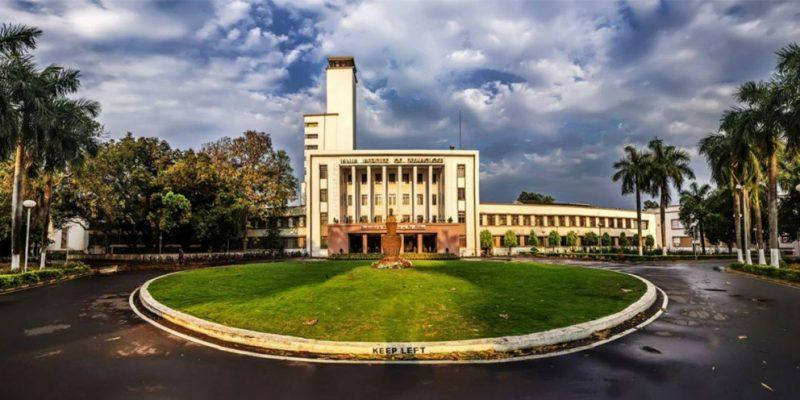
\includegraphics[width=120mm]{Chapter_intro/figs/img1}}
	\caption{Caption of Figure} \label{figure:labelName}
\end{figure}

\section{Research Issues}
List the issues here.

\section{Research Objectives}

This thesis objectives can be listed as follows:

\begin{itemize}
	\item obj1
	\item obj2
	\item obj3
\end{itemize}

\section{Contributions}
The main contributions of this thesis can be summarized as follows:
\begin{itemize}
	\item \textbf{Developed XYZ:} Say something here.
	\item \textbf{Creation of PQR:} Text here.
\end{itemize}

\section{Thesis Organization}

\section{Conclusions}
Summary of the chapter goes here
	\chapter[Conclusions from the Thesis and Future Research Directions]{Conclusions from the Thesis and Future Research Directions}{Conclusions from the Thesis and Future Research Directions}
\label{chap:conclusion}


{\Huge \calligra T}his thesis 
\end{spacing}

%---------------------------------------------------------------
%----------------------- Appendix ------------------------------
%---------------------------------------------------------------
%\begin{comment}
%\renewcommand{\chaptername}{Appendix} %%%%%%%%%%%%%%%%%%%%%%%%%
\begin{appendices}
%%%%%%%%%%%%%%%%%%%%%%%%%%%% APPENDIX %%%%%%%%%%%%%%%%%%%%%%%%%
%\renewcommand{\thesection}{A.\arabic{section}}
\chapter{Appendix 1}{Appendix 1}
\label{App:Appendix1}
\renewcommand{\thesection}{A.\arabic{section}}

\section{Appendix Section 1} 
Text 2.

\section{Appendix Section 2}
Text 2.
\clearpage{\pagestyle{empty}\cleardoublepage}
%\cleardoublepage
\chapter{Appendix-2 Title}{Appendix-2 Title}
\label{App:Appendix2}
\renewcommand{\thesection}{B.\arabic{section}}
\clearpage{\pagestyle{empty}\cleardoublepage}
%\cleardoublepage
\end{appendices}
\renewcommand{\chaptername}{Chapter} %%%%%%%%%%%%%%%%%%%%%%%%%%%%
    \cleardoublepage
    \lhead{} \rhead{}
%\end{comment}
%---------------------------------------------------------------
%----------------------- references ----------------------------
%---------------------------------------------------------------
\addtocontents{toc}{\protect\setcounter{tocdepth}{0}}
\phantomsection
\addcontentsline{toc}{chapter}{Bibliography} %Supress Reference subsection
\chapter*{Bibliography}
\renewcommand{\section}[2]{}% to remove the references heading
\bibliographystyle{IEEEtran}
\renewcommand{\chaptername}{}
\bibliography{RefFile1, RefFile2}
\cleardoublepage
%----------------------------------------------------------------
%---------------------- publication -----------------------------
%----------------------------------------------------------------
\addtocontents{toc}{\protect\setcounter{tocdepth}{2}} %Reinstate level-2 TOC
\phantomsection
\addcontentsline{toc}{chapter}{Publications}
\chapter*{Publications from the Thesis}

\subsection*{Patent Filed}
\begin{enumerate}
	\item{A. Routray, A. Naha, \textbf{A. K. Samanta}, Amey Pawar, \& Chandrasekhar Sakpal, “A system for assessment of multiple faults in induction motors”, WO2019167086A1, 2019.}
\end{enumerate}

\subsection*{Journals}
\begin{enumerate}
	\item{\textbf{A. K. Samanta}, A. Routray, S.R. Khare, \& A. Naha, “Minimum Distance-based Detection of IncipientInduction Motor Faults using Rayleigh Quotient Spectrum of Conditioned Vibration Signal [Accepted]”, \textit{IEEE Transactions on Instrumentation and Measurement.}}
	\item{\textbf{A. K. Samanta}, A. Routray, S.R. Khare, \& A. Naha, “Direct Estimation of Multiple Time-varying Frequencies of Non-stationary Signals”, \textit{Signal Processing}, vol.169, 2020.}
	\item{\textbf{A. K. Samanta}, A. Naha, A. Routray, \& A. K. Deb “Fast and accurate spectral estimation for online detection of partial broken bar in induction motors”, \textit{Elsevier Mechanical Systems and Signal Processing}, vol. 98, pp. 63-77, 2018.}
\end{enumerate}
\cleardoublepage
%----------------------------------------------------------------
%---------------------- biodata ---------------------------------
%----------------------------------------------------------------
\begin{spacing}{1.25}
\phantomsection
\addcontentsline{toc}{chapter}{Author Biography}
\chapter*{Author Biography}

\vspace*{0.15\textheight}

{\em Anik Kumar Samanta} has received his M.S. degree from Indian Institute of Technology Kharagpur in 2016, and his B. Tech. degree from Dr. B. C. Roy Engineering College, Durgapur, India, in 2011. He was also associated with the Center for Railway Research for designing diagnostics of induction motors for the Indian Railways. Currently, he is pursuing his doctoral degree in signal processing at IIT Kharagpur. His research interests include high-resolution spectral estimation, signal-based fault diagnosis of induction motors, detection theory, detection and estimation of parameters under non-stationary conditions, and embedded signal processing. \noindent \textbf{Homepage}: \href{https://eceanik.github.io/}\textbf{{https://eceanik.github.io/}}

\cleardoublepage
\end{spacing}
%----------------------------------------------------------------
%-------------------------- END ---------------------------------
%----------------------------------------------------------------
%================================================================
%======================= Finish =================================
%================================================================
\end{document}